% -----------------------------*- LaTeX -*------------------------------
\documentclass[12pt]{report}
\usepackage{%
	amsfonts,%
	amsmath,%	
	amssymb,%
	amsthm,%
	algorithm,%
%	babel,%
	bbm,%
	etex,%
	%biblatex,%
	caption,%
	centernot,%
	color,%
	dsfont,%
	enumerate,%
	epsfig,%
	epstopdf,%
	geometry,%
	graphicx,%
	hyperref,%
	latexsym,%
	mathtools,%
	multicol,%
	pgf,%
	pgfplots,%
	pgfplotstable,%
	pgfpages,%
	proof,%
	psfrag,%
	subfigure,%	
	tikz,%
	ulem,%
	url%
}	
\usepackage[noend]{algpseudocode}
\usepackage[mathscr]{eucal}
\usepgflibrary{shapes}
\usetikzlibrary{%
  	arrows,%
	backgrounds,%
	chains,%
	decorations.pathmorphing,% /pgf/decoration/random steps | erste Graphik
	decorations.text,%
	matrix,%
  	positioning,% wg. " of "
  	fit,%
	patterns,%
  	petri,%
	plotmarks,%
  	scopes,%
	shadows,%
  	shapes.misc,% wg. rounded rectangle
  	shapes.arrows,%
	shapes.callouts,%
  	shapes%
}

\theoremstyle{plain}
\newtheorem{thm}{Theorem}[section]
\newtheorem{lem}[thm]{Lemma}
\newtheorem{prop}[thm]{Proposition}
\newtheorem{cor}[thm]{Corollary}

\theoremstyle{definition}
\newtheorem{defn}[thm]{Definition}
\newtheorem{conj}[thm]{Conjecture}
\newtheorem{exmp}[thm]{Example}
\newtheorem{assum}[thm]{Assumption}
\newtheorem{axiom}[thm]{Axiom}

\theoremstyle{remark}
\newtheorem{rem}{Remark}
\newtheorem{note}{Note}
\newtheorem{fact}{Fact}

\newcommand{\norm}[1]{\left\lVert#1\right\rVert}
\newcommand{\indep}{\!\perp\!\!\!\perp}
\DeclarePairedDelimiter\abs{\lvert}{\rvert}%
\newcommand\numberthis{\addtocounter{equation}{1}\tag{\theequation}}
\newcommand{\tr}{\operatorname{tr}}
\newcommand{\R}{\mathbb{R}}
\newcommand{\N}{\mathbb{N}}
\newcommand{\E}{\mathbb{E}}
\newcommand{\Z}{\mathbb{Z}}
\newcommand{\B}{\mathscr{B}}
\newcommand{\C}{\mathcal{C}}
\newcommand{\T}{\mathscr{T}}
\newcommand{\F}{\mathcal{F}}
\newcommand{\G}{\mathcal{G}}
%\newcommand{\ba}{\begin{align*}}
%\newcommand{\ea}{\end{align*}}
\newcommand{\expect}[1]{\mathbb{E}\left[{#1}\right]}
\newcommand{\prob}[1]{\mathbb{P}\left[{#1}\right]}
\newcommand{\probo}[1]{\mathbb{P}_0\left[{#1}\right]}
\newcommand{\probi}[1]{\mathbb{P}_1\left[{#1}\right]}
\newcommand{\given}{\; \big\vert \;} 
\newcommand{\bydef}{:=}
\newcommand{\indic}[1]{\mathbbm{1}\{#1\}}
\DeclareMathOperator*{\argmax}{arg\,max}
\renewcommand{\qedsymbol}{$\blacksquare$}
\makeatletter
\def\BState{\State\hskip-\ALG@thistlm}
\makeatother

\makeatletter
\def\th@plain{%
  \thm@notefont{}% same as heading font
  \itshape % body font
}
\def\th@definition{%
  \thm@notefont{}% same as heading font
  \normalfont % body font
}
\makeatother
\date{}
\usepackage{graphicx}
\graphicspath{ {Figures/} }
\usepackage{scribe_e1244}
\usepackage{times}
%\newtheorem{defn}[thm]{Definition}
%\newtheorem{lem}{Lemma}[thm]
%\newenvironment{definition}[1][Definition]{\begin{trivlist}
%\item[\hskip \labelsep {\bfseries #1}]}{\end{trivlist}}
\begin{document}
	\lecturer{Aditya Gopalan}		
	\scribe{Astha Singh \& Varadaraj M.S.}	% required, put your name here
	\lecturenumber{9}			% required, must be a number
	\lecturedate{February 2}		% required, omit year
	\maketitle
	
	% title of the lecture
	\begin{center}
		{\Large \bf Signal Detection in Discrete Time}
	\end{center}
	
	
	% ----------------------------------------------------------------------
	\section{Introduction}
	In this lecture we will learn to apply the binary hypothesis-testing principles, to derive optimum procedures for detecting signals embedded in noise. Let's consider the case of discrete-time detection.
	
	\section{Signal Detection Models and Detector Structures}
	The statistical model we consider has the observation one of the two possible discrete time signals, (with $n$ samples) corrupted by additive noise.
	Thus the observation vector $\underline Y$ is,
	\begin{align*} \underline Y = (Y_1,Y_2, \ldots ,Y_n)^T  \quad  Y\in \Re^n ,
	\end{align*}
	
	$\underline N$ is a vector of noise samples,
	\begin{align*}
	\underline N &= (N_1, \cdots N_n)^T , \\
	\end{align*}
	
	And, $\underline S_0$ and $\underline S_1$ are vectors of samples from the two possible signals,
	\begin{align*}
	\underline S_o &= (S_{01}, \ldots S_{0n})^T\\
	\underline S_1 &= (S_{11}, \ldots S_{1n})^T .\\
	\end{align*}
	
	The hypothesis pair is,
	\begin{align*}
	H_o: Y_k &= S_{0k}+N_k \quad k \in [n]\\
	&\text{vs}\\
	H_1: Y_k &= S_{1k} + N_k \quad k \in [n]\\
	\text{where } [n] &\equiv 1,2,\ldots,n.
	\end{align*}
	
	Typically, the noise $\underline N$ is independent of the signals $\underline S_0 $ and $\underline S_1$, and we work with this assumption throughout.\\
	Now there are three cases:
	\begin{itemize}
		\item {$\underline S_0$ and $\underline S_1$ are deterministic and known}
		\item {$\underline S_0$ and $\underline S_1$ are partially deterministic and partially random}
		\item {$\underline S_0$ and $\underline S_1$ are completely random}
	\end{itemize}
	
	\subsection{Detection of Deterministic Signals in Independent Noise}
	The two signals $S_0$ and $S_1$ are completely deterministic. We have $\underline S_j = \underline s_j$, with $\underline s_j \in \Re ^n$ being known to the designer. This is also known as the \textit{coherent} detection problem.\\
	\begin{assum}
	$N_1$ , $N_2$ ,\ldots , $N_n$ are independent.
	\end{assum}
	
	\noindent The likelihood ratio of an observation $\underline y$ $\in$ $\Re^n $ is:
	
	\begin{align*}
    L(y) &= \frac{p_1(y)}{p_0(y)}\\
    &= \frac{p_{\underline N}( \underline y - \underline s_1)}{p_{\underline N}( \underline y - \underline s_0)} \quad
    \text{where,}p_{\underline N}(x)  \text{: Probability density of \underline N at x}\\
    &= \frac{p_{N_1}(y_1 - s_{11}).p_{N_2}(y_2 - s_{12}) \ldots p_{N_n}(y_n - s_{1n})}{p_{N_1}(y_1 - s_{01}).p_{N_2}(y_2 - s_{02}) \ldots p_{N_n}(y_n - s_{0n})}\\
    &= \prod_{k=1}^{n} \frac{p_{N_k}(y_k-s_{1k})}{p_{N_k}(y_k-s_{0k})}\\
    &\bydef \prod_{k=1}^{n} L_k(y_k)
\end{align*}

	\noindent An optimum detector (Bayes, Minmax, Neyman-Pearson) has the form:\\
	\begin{align*}
	\delta(y)=
	\begin{cases}
	1, \quad \text{if } & > \\
	\gamma, \quad \text{if } \sum_{k=1}^{n}log L_k(y_k) &= log \tau \\
	0, \quad \text{if } & < 
	\end{cases}
	\end{align*}
	
	
	\begin{figure}[h]
		\centering
		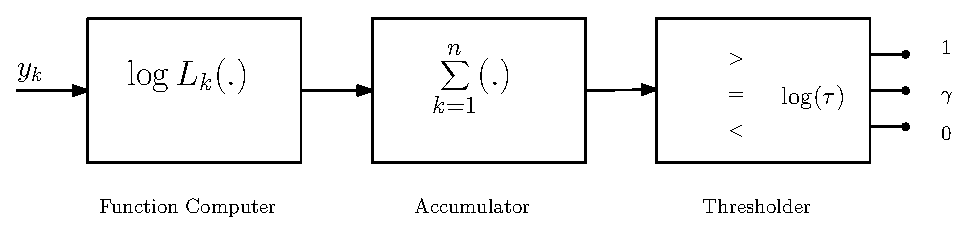
\includegraphics[scale=1.0]{Figures/CohDetector.eps}
		\caption{Detector Structure : Coherent Detection in Independent Noise}
		\label{fig:CohDetector}
	\end{figure}
	
	\noindent As illustrated in Figure 9.1, this structure consists of a time-varying instantaneous non-linearity $log L_k$ , followed by an accumulator, that is in turn followed by a threshold comparator.
	
	
	\begin{exmp}[Coherent Detection in iid (independent and identically distributed) Gaussian Noise]
	
		$$ (N_1,N_2,...,N_n) \sim \mathcal{N}(0,\sigma^2) $$
		\begin{assum}
		
		\begin{align*}
		\underline s_0 &= \underline 0 \quad \in \Re ^n\\
		\underline s_1 &= \underline s \quad \in \Re ^n
		\end{align*}
		This assumption does not result in any loss in generality since we could always redefine our observations as $\underline y' = \underline y - \underline s_0 $ so that the signal would be \underline{0} under $H_0$ and $\underline s = \underline s_1 - \underline s_0 $ under $H_1$.
		
	    \end{assum}
		
		Computing $L_k(y_k)$:
		\begin{align*}
		log L_k(y_k) &= log \frac{\exp {- \frac{(y_k-s_k)^2}{2 \sigma ^2}}}{\exp {- \frac{(y_k-0)^2}{2 \sigma ^2}}}\\
		&= \frac{1}{2 \sigma ^2}(y_k^2 - (y_k-s_k)^2)\\
		&= s_k (y_k- \frac{s_k}{2}) \frac{1}{\sigma ^2}
		\end{align*}
		
		The optimum detector is:
		
	\begin{align*}
\delta(y) &=
\begin{cases}
1, \quad \text{if} \quad\sum_{k=1}^{n}s_k(y_k - \frac{s_k}{2}) > \tau ' \\
\gamma, \quad \text{if}\quad \sum_{k=1}^{n}s_k(y_k - \frac{s_k}{2}) = \tau '  \\
0, \quad \text{if} \quad\sum_{k=1}^{n}s_k(y_k - \frac{s_k}{2}) < \tau '
\end{cases}\\
\text{where, } \tau ' & \bydef \sigma ^2 log \tau \\
& \Rightarrow
\begin{cases}
1, \quad \text{if} \quad\sum_{k=1}^{n}s_k y_k > \tau '' \\
\gamma, \quad \text{if} \quad \sum_{k=1}^{n}s_k y_k = \tau ''  \\
0, \quad \text{if} \quad \sum_{k=1}^{n}s_k y_k < \tau ''
\end{cases}\\
\text{where, } \tau '' & \bydef \tau ' + \frac{1}{2} \sum_{k=1}^{n} s_k^2
\end{align*}
\noindent This optimum detector structure is depicted in Figure 9.2 and is known as {\em Matched Filter} Detector.
		
		\begin{figure}[h]
			\centering
			\includegraphics[scale=0.9]{Figures/MatchedDetector.eps}
			\caption{Optimum detector for coherent signals i.i.d Gaussian noise.}
			\label{fig:MatchedDetector}
		\end{figure}
	\end{exmp}
	
	\begin{exmp}[Coherent Detection in iid Laplace Noise]
		Here also the noise samples $N_1, \ldots ,N_2$ are i.i.d, but with Laplacian marginal probability density,
		\begin{align*}
		p_{N_k}(x) &= \frac{\alpha}{2}e^{-\alpha |x|}\\
		\text{where, } \alpha >0 &: \text{a constant}
		\end{align*}
		This model is sometimes used to represent the behaviour of impulsive noises in communication receivers.
		
		Computing $L_k(y_k)$:
		\begin{align*}
		log L_k(y_k) &= log \frac{e^{- \alpha |y_k-s_k|}}{e^{- \alpha |y_k|}}\\
		&= \alpha (|y_k|-|y_k-s_k|)
		\end{align*}
		
		\begin{figure}[h]
			\centering
			\includegraphics[scale=0.6]{Figures/Sk_greaterthanzero.eps}
			\caption{$S_k>0$}
			\label{fig:Sk_greaterthanzero}
		\end{figure}
		
		\begin{figure}[h]
			\centering
			\includegraphics[scale=0.6]{Figures/Sk_lessthanzero.eps}
			\caption{$S_k<0$}
			\label{fig:Sk_lessthanzero}
		\end{figure}
		
		This function $log L_k(y_k)$ is depicted in Figure 9.3 and Figure 9.4 for both cases $ s_k<0$ and $s_k>0$ respectively.
		
		We now define $l_k(x)$ as:
		
		\begin{align*}
		l_k(x)=
		\begin{cases}
		- \frac{|s_k|}{2} &\text{if} \quad x \leq - \frac{|s_k|}{2}\\
		\quad x &\text{if} \quad \frac{-|s_k|}{2} < x \leq \frac{|s_k|}{2}\\
		\quad\frac{|s_k|}{2} &\text{if} \quad x > \frac{|s_k|}{2}
		\end{cases}
		\end{align*}
		
		This function is sometimes known as a \textit{Soft Limiter}, Figure 9.5.
		
		\begin{figure}[h]
			\centering
			\includegraphics[scale=0.6]{Figures/SoftLimiter.eps}
			\caption{Soft Limiter}
			\label{fig:SoftLimiter}
		\end{figure}
		
		\begin{equation}
		log L_k(y_k) = 2 \alpha sign(S_k) l_k(y_k - \frac{S_k}{2})
		\end{equation}
		
		
		Thus the optimal detector is:
		
		\begin{align*}
		\delta(y)=
		\begin{cases}
		1, \quad \text{if} &> \\
		\gamma, \quad \text{if} \quad\sum_{k=1}^{n} sign(s_k) l_k(y_k- \frac{s_k}{2}) &= \tau ' \\
		0, \quad \text{if} &< 
		\end{cases}
		\end{align*}
	
		\begin{figure}[h]
			\centering
			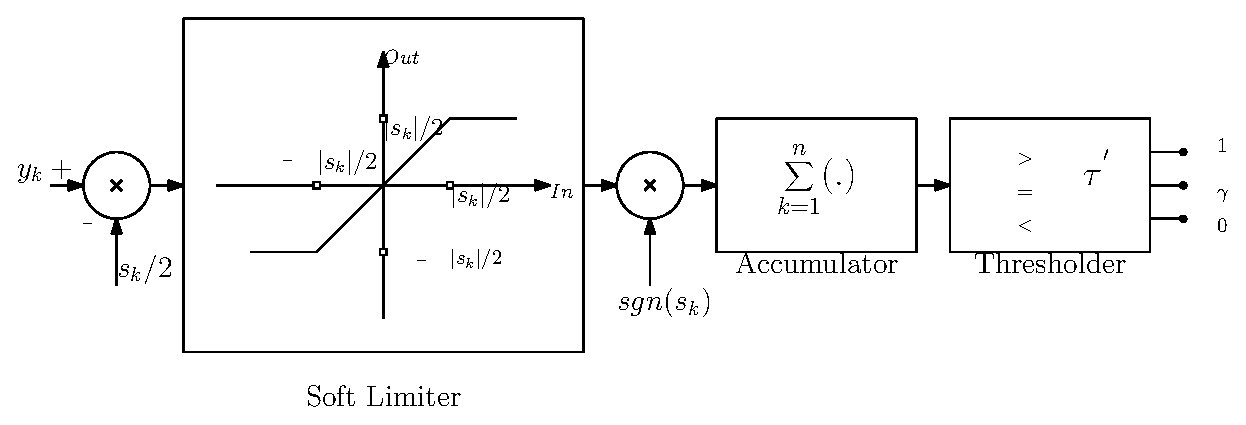
\includegraphics[scale=0.6]{Figures/SoftLimiterDet.eps}
			\caption{Soft Limiter Detector}
			\label{fig:SoftLimiterDet}
		\end{figure}
	\end{exmp}
	
	Thus this detector system "centers" the observations by subtracting $s_k/2$ from each $y_k$. It then correlates the centered(\text{soft-limited}) data with the known signal and compares the output of this correlation with a threshold. It has the effect of making the system more tolerant to large noise values.
	
	\subsection
	{Locally Optimum Detection of Coherent Signals in i.i.d. Noise}
	 
	While detecting signals, the expected structure or form  of the received signal is often known and it's amplitude is unknown. Such a problem is modelled using {\em composite hypothesis-testing} described by
	\begin{align*}	
	&H_{0}: Y_{k} = N_{k}, \quad  k \in [n],\\
	&H_{1}: Y_{k} = N_{k}+\theta{s_{k}}, \quad  k \in [n],\hspace{10pt}\theta>0,
	\end{align*}
	
	\begin{assum}
		$\underline{s}=(s_{1},...,s_{n})^T$ is a known signal.
	\end{assum}
	
	\begin{assum} $\underline{N}=(N_{1},...,N_{n})^T$ is a continuous random vector with i.i.d. components and marginal probability density functions $p_{N_{k}}$, where $\theta$ is the parameter generally associated with attenuation.
	\end{assum}
	\noindent Hence the distribution is
	\begin{align*}
	&\Lambda = [0, \infty)\\
	&\Lambda_0 = \{0\} , \ \Lambda_1 = (0, \infty)
	\end{align*}
	
	\begin{defn}
		\noindent The critical region for testing $H_0$ v/s $H_1$ is: $\Gamma_{\theta}=\{\underline{y}\in{\rm I\!R}^n|L_{\theta}(\underline{y})>\tau\}$.
	\end{defn}
	
	\begin{note}
		You can always subtract one from another. Hence testing  $H_0$ v/s $H_1$ simplifies to testing \{0\} v/s $\{\theta\}$.  
	\end{note}
	
	\begin{note} 
		If the critical region depends on $\theta \in \Lambda_1$ then there cannot exist a UMP (Uniformly Most Powerful) test. Hence UMP test exists only for particular noise models.
	\end{note}
	
	\begin{note}
		However LMP (Locally Most Powerul) tests have a simple and inherently reasonable structure, and thus it is of interest to consider locally optimum detection for this case.
	\end{note}
	
	\subsection{LMP test}
	
	\par A LMP test is of the form:
	\begin{equation}
	\delta_{LMP}(y)=\begin{cases}
	1&>\\
	\gamma \quad\text{if }\frac{\partial}{\partial\theta}P_{\theta}(\underline{y})\big|_{\theta=0}&=\tau P_{0}(\underline{y}).\\
	0&<
	\end{cases}
	\end{equation}
	
	\begin{equation}
	\frac{\partial}{\partial\theta}L_{\theta}(\underline{y})\big|_{\theta=0}\quad\gtreqqless\quad \tau
	\end{equation}
	
	Upon differentiation, we have
	\begin{eqnarray}
	\frac{{\partial}}{\partial\theta}L_{\theta}(\underline{y})\hspace{2pt}|_{\theta=0}&=&\frac{\partial}{\partial\theta}\left(\prod_{k=1}^n\frac{p_{N_{1}}(y_{k}-\theta{s_{k}})}{p_{N_{1}}(y_{k})}\right)\hspace{2pt}\Bigg|_{\theta=0}\nonumber\\
	&=&\left(\prod_{k=1}^n\frac{p_{N_{1}}(y_{k}-\theta{s_{k}})}{p_{N_{1}}(y_{k})}\right)\left(\sum_{k=1}^{n}\frac{\frac{\partial}{\partial\theta}p_{N_{1}}(y_{k}-\theta{s_{k}})}{p_{N_{1}}(y_{k}-\theta{s_{k}})}\right)\Bigg|_{\theta=0}\nonumber\\
	&=&\sum_{k=1}^{n}\frac{-s_{k}p_{N_{1}}^\prime(y_{k}-\theta{s_{k}})}{p_{N_{1}}(y_{k}-\theta{s_{k}})}\Bigg|_{\theta=0}\nonumber\\
	&=&\sum_{k=1}^{n}s_{k}\left(\frac{-p_{N_{1}}^\prime(y_{k})}{p_{N_{1}}(y_{k})}\right)\nonumber\\
	&=&\sum_{k=1}^{n}s_{k}g_{lo}(y_{k})
	\end{eqnarray}
	
	\noindent where the second equality is obtained by the modified version of chain rule of differentiation
	
	\begin{eqnarray}
	\frac{{dv}}{d\theta}(f(\theta).g(\theta))&=& f(\theta).g^{'}(\theta)+f^{'}(\theta).g(\theta)\nonumber\\
	&=&f(\theta).g(\theta)\left\{\frac{g^{'}(\theta)}{g(\theta)} + \frac{f^{'}(\theta)}{f(\theta)}\right\}
	\end{eqnarray}
	 
	\noindent where $g_{lo}(y)\triangleq-\ p_{N_{1}}^\prime(y)/p_{N_{1}}(y)$, where $p_{N_{1}}^\prime(y)=dp_{N_{1}}(y)/dy.$ Structure  depicted in Figure(\ref{fig:loc_opt_detector})
	
	\begin{figure}[h]
		\centering
		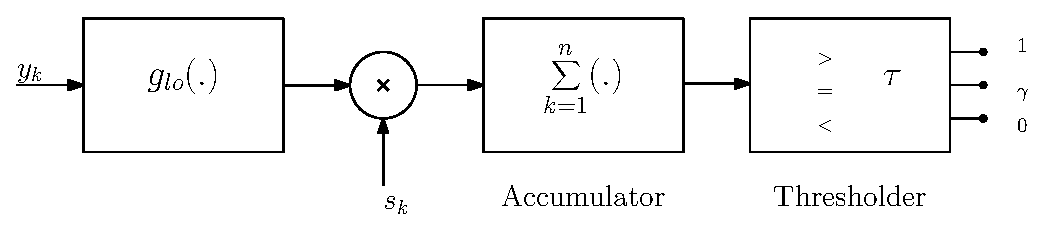
\includegraphics[scale=0.7]{Figures/loc_opt_detector.eps}
		\caption{Locally optimum detector structure for coherent signals in i.i.d noise}
		\label{fig:loc_opt_detector}
	\end{figure}
	
	 \noindent (Note:Similar to likelihood ratio the locally optimum nonlinearity $g_{lo}$ shapes the observation to reduce the ill effects of noise.)
	
	\begin{exmp}
		 For Standard Gaussian noise $\mathcal{N}(0,\sigma^2)$, we have
		\begin{eqnarray}
		g_{lo}(y)&=& 
		\frac{-\frac{1}{\sigma.\sqrt{2\pi}}e^{-(y^2)/2\sigma^2}.\frac{-2y}{2\sigma^2}}{\frac{1}{\sigma.\sqrt{2\pi}}e^{-(y^2)/2\sigma^2}}\\&=&\frac{y}{\sigma^2}
		\end{eqnarray}
		\par Hence the locally optimum detector structure is simply the correlation detector.
	\end{exmp}
	
	\begin{exmp} For Standard laplacian noise with density $p_{N1}(y) = \frac{\alpha}{2}e^{-\alpha |y|}$, we have
		\begin{eqnarray}
		g_{lo}(y)&=& \frac{p_{N_{1}}^\prime(y)}{p_{N_{1}}(y)}\\
		&=&
		\begin{cases}
		\alpha&if \quad y > 0\\
		 0&if \quad y=0\\
		{-\alpha}&if \quad y < 0
		\end{cases}
		\end{eqnarray}
		
		\par we have $g_{lo}(y)$ = $\alpha sign(y),$ So the locally optimum detector correlates the signal with the sequence of signs of the observations. The function  $g_{lo}(y)$ in this case is known as a \textbf{\textit{hard limiter}}(Figure\ref{fig:Hard Limiter}).
		
		\begin{figure}[h]
			\centering
			\includegraphics[scale=0.6]{Figures/HardLimiter.eps}
			\caption{Locally optimum non linearity for standard Laplacian noise}
			\label{fig:Hard Limiter}
		\end{figure}
	\end{exmp}
	
\end{document}